% !TEX TS-program = pdflatex
% !TEX encoding = UTF-8 Unicode

% This is a simple template for a LaTeX document using the "article" class.
% See "book", "report", "letter" for other types of document.

\documentclass[12pt]{article} % use larger type; default would be 10pt

\usepackage{csvsimple}
\usepackage{booktabs}  % For nicer table formatting

\usepackage{KUstyle}

\usepackage[utf8]{inputenc} % set input encoding (not needed with XeLaTeX)

\usepackage{graphicx} % required for inserting images

%%% Examples of Article customizations
% These packages are optional, depending whether you want the features they provide.
% See the LaTeX Companion or other references for full information.

%%% PAGE DIMENSIONS
\usepackage{geometry} % to change the page dimensions
\geometry{a4paper} % or letterpaper (US) or a5paper or....
\usepackage{setspace}
\usepackage{parskip}
\parskip=1\baselineskip %\advance\parskip by 0pt plus 2pt% to change between paragraphs space
% \geometry{margin=2in} % for example, change the margins to 2 inches all round
% \geometry{landscape} % set up the page for landscape
%   read geometry.pdf for detailed page layout information

% \usepackage{gravarphicx} % support the \includegravarphics command and options

% \usepackage[parfill]{parskip} % Activate to begin paragraphs with an empty line rather than an indent

%%% PACKAGES
\usepackage{booktabs} % for much better looking tables
\usepackage{array} % for better arrays (eg matrices) in maths
\usepackage{paralist} % very flexible & customisable lists (eg. enumerate/itemize, etc.)
\usepackage{verbatim} % adds environment for commenting out blocks of text & for better verbatim
\usepackage{subfig} % make it possible to include more than one captioned figure/table in a single float
% These packages are all incorporated in the memoir class to one degree or another...
\usepackage[fleqn]{amsmath}
\usepackage{amssymb}
\usepackage{enumitem}
\usepackage{amsthm}
\usepackage{graphicx}
\usepackage{filecontents}
\usepackage{natbib}
\usepackage{scrextend}
\usepackage[table,xcdraw]{xcolor}
\usepackage{tabularx}
% If you use beamer only pass "xcolor=table" option, i.e. \documentclass[xcolor=table]{beamer}
\usepackage{lscape}
\usepackage{longtable}
\usepackage{booktabs}
\usepackage{subcaption}
\usepackage{amsmath}


%%% Customizing
\DeclareMathOperator*{\argmax}{arg\,max}
\DeclareMathOperator*{\argmin}{arg\,min}




%%% HEADERS & FOOTERS
\usepackage{fancyhdr} % This should be set AFTER setting up the page geometry
\pagestyle{fancy} % options: empty , plain , fancy
\renewcommand{\headrulewidth}{0pt} % customise the layout...
\lhead{}\chead{}\rhead{}
\lfoot{}\cfoot{\thepage}\rfoot{}


%%% Author superscript
    \makeatletter
\def\@fnsymbol#1{\ensuremath{\ifcase#1\or\ast\or \dagger\or \ddagger\or
   \mathsection\or \mathparagraph\or \|\or **\or \dagger\dagger
   \or \ddagger\ddagger \else\@ctrerr\fi}}
    \makeatother


%%% SECTION TITLE APPEARANCE
\usepackage{sectsty}
\allsectionsfont{\rmfamily\bfseries\upshape} % (See the fntguide.pdf for font help)
% (This matches ConTeXt defaults)

\usepackage[nottoc,notlof,notlot]{tocbibind} % Put the bibliography in the ToC
\usepackage[titles,subfigure]{tocloft} % Alter the style of the Table of Contents
\renewcommand{\cftsecfont}{\rmfamily\mdseries\upshape}
\renewcommand{\cftsecpagefont}{\rmfamily\mdseries\upshape} % No bold!

\usepackage[colorlinks,citecolor=black,urlcolor=black,bookmarks=false,hypertexnames=true]{hyperref} 
%%% END Article customizations
%%% The "real" document content comes below...


% This changes the content of the front page
\ptype{Course Project}
\title{Predicting Housing Prices in Denmark -- A Machine Learning Approach}
\author{Group 23: He SHI, Mingjie XING, Qi ZHANG}
\date{Submitted: \today} % Activate to display a given date or no date (if empty),
         % otherwise the current date is printed 
\keystrokes{Keystrokes: {... (... normal pages)}}
\contribution{Member contribution:\\
He SHI: 1 Introduction, 3.2 Data scraping, 3.3 Analysis of scraping log and 3.6 Key statistics;\\ 
Mingjie XING: 3.5 Data validation, 4 Methods, 5 Empirical analysis and 7 Conlusion;\\
Qi ZHANG: 2 Literature Review, 3.1 Data Ethics, 3.4 Data preprocessing, 6 Discussion.}


\renewcommand{\contentsname}{Table of content}






\begin{document}

\maketitle

% table of contents
\newpage

\tableofcontents
\newpage

{\fontfamily{ptm}\selectfont

\pagenumbering{arabic}


\section{Introduction}
        The evolution of the Danish real estate market over the past decade underscores the interplay of diverse factors that have influenced property prices. The market demonstrates resilience and regains momentum soon after crises, even facing the initial impact of the COVID-19 pandemic. By the early 2010s, the market had rebounded from the financial crisis, benefiting from favorable economic conditions and historically low-interest rates. This, coupled with steady housing demand, led to moderate price growth. Notably, Copenhagen experienced a surge in property prices driven by urbanization trends and heightened demand.

        Around 2017, moderation in price growth emerged as tighter lending regulations were enforced to prevent housing bubbles. Additionally, measures were introduced to curtail speculative investing, resulting in a more balanced market environment. Despite pandemic-related uncertainties, the market showcased adaptability and regained stability, with persistent strong demand in urban centers. Nevertheless, efforts to ensure affordability and curb overheating influenced the trajectory of price growth.

        Examining the factors influencing real estate prices remains pertinent. We intend to utilize current data from \url{https://www.boligsiden.dk/} to conduct a detailed analysis of price changes using machine learning models. This approach will shed light on the complex interplay of elements shaping the market, contributing to a comprehensive understanding of real estate dynamics and facilitating informed decision-making.


        \begin{figure}[h]
            \centering
            \includegraphics[width=15cm, height=7cm]{fig/price.png}
            \caption{real estate price change over time (globalpropertyguide.com)}
            \label{fig:price}
        \end{figure}

        When we click on a property link on \url{https://www.boligsiden.dk/}, we uncover a wealth of valuable details about that property. This encompasses key aspects like location, size, and price. Additionally, an introduction provides insights into the property's unique features. We can also track the property's price changes, compare it with neighboring properties, and gauge recent interest. Public comments offer communal perspectives, and internet connectivity data offers practical insight. Hyperlinks reveal even more hidden treasures. They provide access to broader price trends and more detailed information. Focusing on our analysis, we require specific information. Our main target is residential property prices, and we're also interested in fundamental property data like size and location. In addition, we leverage energy rankings and days after sale as valuable context to our analysis. This curated collection of data elements forms the cornerstone of our exploration, allowing us to gain insights into real estate dynamics.

        We trained a 3-degree polynomial regression with LASSO regularization and a gradient-boosting model to predict housing prices with the features we scraped from the website. For the boosting model, we experimented three scikit-learn functions, which have different attributes, i.e., \texttt{GradientBoostingRegressor}, \texttt{HistGradientBoostingRegressor}, and \texttt{XGBRegressor}. For all models we conducted 10-fold cross-validation. Our research shows that a tuned extreme gradient boosting model can best predict housing prices with an R2 score of 44\% and Root mean squared errors (RMSE) of 2,329,683.66. 
        				

\section{Literature Review}
\subsection{Housing Price Prediction by Machine Learning Models}
		There are several papers recently in top journals in real estate economics predicting housing prices with machine learning models: 		\cite{Deppneretal2023} applies a non-parametric machine learning model with k-fold cross-validation to examine the U.S. commercial real estate appraisal to shrink the deviations between market values and subsequent transaction prices.	\cite{Linetal2023} augments the traditional hedonic model with the Gradient Boosting Machine algorithm to predict housing prices in Beijing. \cite{TchuenteNyawa2022} uses artificial neural networks, random forest, adaptive bBoosting, gradient boosting, and K-nearest neighbors algorithms to estimate real estate prices in French cities. Real estate price prediction is challenging and attracts ongoing research. 

        \cite{mohdetal2020} reviews techniques like Neural Networks, Hedonic Price Model, SVM, Linear Regression, Decision Tree, Random Forest, KNN, Fuzzy Logic, among others, for property price forecasting. These studies have provided substantial evidence to support the notion that machine learning models are capable of accurately predicting house prices. 
\subsection{Independent Variables for House Price Prediction} 
        When examining specific independent variables for house price, researchers commonly choose a range of factors to demonstrate changes in house prices. This diverse selection reflects the understanding that various influences affect the housing market. These key variables includes: \cite{girouardetal2001} uses economic indicators, \cite{engelhardtetal1991} uses demographics, \cite{gelfandetal2004} uses location, and \cite{caseetal1991} uses property attributes, all offer a comprehensive view of the intricate relationship between factors and the dynamic nature of house prices. \cite{paceetal1998} uses the characteristics or variables affecting housing prices can be classified according to different criteria, and the classical specification of feature models namely structural features and positional features.  \cite{chicaetal2013} indicates that the price of the house mainly depends on the nearby housing prices.
\subsection{Distinct Factors in Denmark House Prices}
        For Denmark house prices, the studies show us the influencing factors are slightly different from other countries. \cite{englundetal1997} examines house price trends in 15 OECD nations, uncovering remarkable similarities among these countries. \cite{marshetal2010} indicates that energy consumption of houses holds considerable significance among individuals in Denmark. Using the hedonic price method, \cite{praestholmetal2002} finds significant and positive homeowner willingness to pay for forest proximity, often surpassing afforestation costs.

  
  
	\subsection{Contribution}
		This project makes significant contributions by: 1) meticulously compiling a comprehensive dataset that encapsulates the intricacies of Denmark's residential real estate market, thereby offering a valuable resource for comprehensive analysis; and 2) constructing a robust predictive model tailored to Denmark's various cities, enabling the accurate anticipation of housing price fluctuations. These achievements collectively aim to deepen insights into the complexities of the housing market and furnish stakeholders and researchers with a reliable framework for informed decision-making and exploration.

		

\section{Data Description}
    We are going to scrape the individual-level house prices from boligsiden.dk, a major real estate broker in Denmark covering housing prices as monthly data of 36 months scale and detailed features of houses in different regions with open data access. Structural features in data include area, location, age, and owner income. Web scraping of the data is allowed for academic use. There will be about 3700 house-month-region observations in our dataset. \par
    
    \subsection{Data Ethics}

        The data used in this project is obtained through web scraping from the Boligsiden platform. This platform provides information about the residential real estate market in Denmark, and thus, the data we have collected to some extent represents the state of the Danish residential real estate market.

        Throughout the process of data collection and utilization, we have consistently adhered to the principles of legal compliance, particularly in accordance with the regulations set forth in the European Union's Digital Services Act (\cite{DecisionServicesAct2022}). This ensures the transparency and legality of our data usage. Moreover, to safeguard individual privacy, the data we have utilized is strictly limited to publicly available information, devoid of any personal sensitive data. When presenting the data, we have employed aggregation techniques to ensure the privacy and anonymity of individual observations.

        Simultaneously, we are committed to upholding the seven principles of the General Data Protection Regulation (GDPR). These principles encompass legality, fairness, transparency, purpose limitation, data minimization, accuracy, and storage limitation. Our data collection and usage adhere to legal boundaries while respecting the rights of data subjects. The purposes of data usage are well-defined, restricted to the objectives of this project, ensuring data accuracy and currency, and placing strict limitations on data retention.

        By adhering to these principles, our aim is to ensure secure, legal, and transparent use of data for valuable research purposes while safeguarding the privacy rights of data subjects.



        \subsection{Data Scraping}
        Our data collection process started on August $15^{th}$ and took about three days to complete. During this time, we faced some challenges. One was making sure that the data we collected from the website matched up correctly. Another challenge was figuring out where exactly to find the different details on the website. But as we worked through these challenges, we actually got better at understanding how websites are structured and how to get the information we need.

        At the outset, we collected details about eleven different property features that we believed could aid in predicting prices. This effort resulted in a dataset containing 3650 entries after cleaning. Initially, we had a list of 10,000 website links (URLs) to work with, which we considered a sufficient number for our analysis. By filtering for links with 'address', we were left with 7619 URLs. However, after investigating errors, we discovered that the main obstacle preventing us from accessing all 7619 URLs was the error message 'NoneType' object has no attribute 'text'". As a result, our dataset consisted of 3754 entries before cleaning, carefully curated to align with our research objectives. Additionally, during our journey, we recognized that certain collected information was not essential for our goals. Consequently, we chose to exclude these irrelevant details from our analysis.
       
        A total of nine features have been deemed pertinent for our analysis. To facilitate our subsequent analysis, we have transformed 'city', 'energy', 'area\_code' and 'type' into dummy variables. This transformation enables us to effectively incorporate these variables into our analytical framework. Numerical variables include 'saledays', 'living\_space', 'ground\_space', 'rooms', 'age'.
       


        \subsection{Analysis of Scraping Logs}
        This section will analyze the logs created in the scraping process, with the intention of ensuring the data quality. Logging during data scraping serves as a fundamental practice to document and monitor the process of retrieving information from websites. It involves capturing relevant details and events throughout the scraping operation and saving them for reference, analysis, and troubleshooting purposes. In our logging process, We mainly acquire the time of scraping, the status code of the request-response, the length of the output, and the path to the output file. 

        \textbf{Response Status Code}
        HTTP status codes logged during the scraping process can indicate the success or failure of requests. Non-200 status codes, such as 404 (Not Found) or 500 (Internal Server Error), may suggest issues with the availability or integrity of the data being accessed.


        \begin{figure}[]
            \centering
            \includegraphics[width=15cm, height=7cm]{fig/response_codes_chart.png}
            \caption{response codes over time}
            \label{fig:response_codes}
        \end{figure}

        As observed in the Figure \ref{fig:response_codes}, the response codes consistently indicate a '200' status. While a total of 7619 requests were initiated, only 5418 of these have been successfully logged. This discrepancy can be attributed to several factors. Firstly, instances of requests timing out may arise due to sluggish or unresponsive servers. Consequently, these instances might result in incomplete responses that remain unrecorded if not adeptly addressed. Secondly, the presence of duplicate URLs within the request list may lead to redundant requests, potentially resulting in incomplete logging if mechanisms to circumvent redundant scraping are not in place. Lastly, it is plausible that the website being scraped enforces rate limiting or other constraints, limiting the number of requests permissible within a short time span.

        \textbf{Response Length and Content}
        The length of the response content logged can offer insights into the amount of data retrieved from the website. Drastic variations in response length across similar requests might indicate irregularities in the website's structure or discrepancies in data presentation.

        \begin{figure}[]
            \centering
            \includegraphics[width=15cm, height=7cm]{fig/response_sizes_chart.png}
            \caption{response sizes over time}
            \label{fig:response_sizes}
        \end{figure}

        \begin{figure}[]
            \centering
            \includegraphics[width=15cm, height=7cm]{fig/response_sizes_distribution.png}
            \caption{response sizes distribution}
            \label{fig:res_size_distr}
        \end{figure}


        Figure \ref{fig:response_sizes} plots response sizes throughout the duration of the web scrapings. The response sizes vary throughout the scrape. Figure \ref{fig:res_size_distr} presents the distribution of response sizes, showcasing a distribution pattern that closely resembles a normal curve. Notably, instances of notably large response sizes are infrequent within this distribution. The presence of inconsistent response sizes for similar requests potentially signifies variations in the content served by the server. Interestingly, our dataset lacks extremely small response sizes, which is often indicative of crucial data or content absent from the response. This indicates that our data collection process has managed to avoid instances of missing information. This absence is a positive aspect as it implies that our scraping process has been effective in capturing relevant data. Conversely, larger response sizes might point to the server transmitting extensive content, potentially encompassing multimedia elements, attachments, or supplementary resources. Scrutinizing the dynamics of response sizes helps provide a comprehensive evaluation of the data quality landscape and allows us to identify patterns or anomalies that might require further investigation.

        \textbf{Response Time}
        Response time, also known as latency, refers to the amount of time it takes for a system, application, or service to respond to a given request. In the context of web scraping and data extraction, response time typically pertains to the duration between sending an HTTP request to a web server and receiving the corresponding response. Response time is a crucial metric in various scenarios and can provide valuable insights into the performance and efficiency of systems and services. 


        \begin{figure}[]
            \centering
            \includegraphics[width=15cm, height=7cm]{fig/response_times_chart.png}
            \caption{response time}
            \label{fig:res_time}
        \end{figure}

        As depicted in Figure \ref{fig:res_time}, the response time distribution generally follows a normal pattern with most responses clustering around the 1-second mark. However, the figure also illustrates two instances of notably large response times. Several reasons can contribute to the occurrence of large response times. Firstly, when the web server faces an influx of requests or experiences heavy traffic, it may need more time to process each request. Consequently, response times can be extended due to the increased load on the server's resources. Secondly, response times can be prolonged when data has to traverse multiple network nodes before reaching the requesting system. Slow network connections or congested routes can introduce delays in data transmission. Thirdly, some websites and APIs enforce rate limits on the number of requests that can be made within a specific time interval. Exceeding these limits can result in lengthened response times as the server restricts the frequency of responses to meet the imposed limits. Understanding the underlying reasons for these large response times is essential for optimizing the web scraping process. 

        In our analysis, it's important to acknowledge certain limitations that affect our ability to pinpoint the exact reasons for large response sizes and extended response times. Due to the absence of request-specific information in our logging file, we are unable to precisely identify the factors leading to these occurrences. However, we have diligently sought to identify potential explanations that enable comprehensive analysis. The graphs presented above play a significant role in shedding light on the quality of the data. Despite the aforementioned limitations, we have effectively demonstrated the data quality through various visualizations and observations. The distribution of response sizes and response times, combined with insights derived from response code analysis, provides valuable indications of the integrity and consistency of the collected data.
    
       
       
        \subsection{Data preprocessing}
        
		The original data after scraping needs to be cleaned for machine learning. 
        
        \textbf{Split 'data' variable}
        Firstly,for the 'data' variable of original database including detailed data,we split it to 'living space', 'ground space', 'rooms', 'owner expenses', and 'year'. The 'living space' includes only those rooms that serve for living, living and residence in the house or apartment. The 'ground space' shows the total area that belongs to the home/plot. The 'owner expenses' are the expenses that the new owner of the home must pay in the first year in addition to interest and installments on the loan. The owner's expenses cover i.a. property value tax, property debt and home insurance as well as expenses for owners' association, renovation etc. But we find out the 'owner expenses' would cause the data leakage problem because the value is estimated from house price. The 'rooms' and and 'year' mean the number of total rooms and the year when the house was built.\par
        
        \textbf{String method}
        We utilize string methods to replace and extract data on the 'city', 'price', and 'saledays' columns.
        
        \textbf{Create dummy variable}
        Then we categorized different types of houses as "Villa," "Apartment," "Terraced house," "Holiday home," and so on, helps simplify the dataset and make it more conducive to analysis and understanding, and created five dummy variables about the house types. We found an independent variable of interest named energy label which is from A to G, indicating how energy efficient the house is. We replaced certain energy labels with a unified category, creating dummy variables for 'energy' columns, and then concatenating these dummy variables with the original dataframe for further analysis. Even though dropping 'none' value processing would drop the observations which do not have an energy label, we still reserve this as a feature because \cite{marshetal2010} shows that people place significant importance on house energy consumption in Denmark. 
        
        \textbf{Other cleaning procedure for ML} For ground space, we replace 'none' with 0 rather than delete them ,because they belong to the 'apartment' and the ground space of the apartment is not in consideration when buying and selling consumption behavior. We convert building year to age for ML. We split 'area' to 'area code' to 'area address' by extracting numbers from 'area name'. Some 'area code' are empty because some postal codes between text, it's populated with the extracted numbers from 'area name'. Using the 'area code' as independent variable would cause the over-fitting problems because the area code is a category rather than a continuous variable, so we exact the first digit of the area code to create it dummy variable. But after practical analysis, we rule out first digit of the area code dummy variable because it can only delicate the zone in Denmark, city dummy variables can be more explanatory. \par

         
         The table of contents and description of each variable is in the appendix. Before the cleaning, we have more than 7600 observations, and after the cleaning, we have 3651 observations. 

        \subsection{Data validation}
            To make sure that the data scraped from the Boligsiden is representative of the residential real estate market in Denmark, we compare scraped data with the average property prices by postal code area in Denmark obtained from Finans Denmark on \url{https://rkr.statbank.dk/statbank5a/default.asp?w=1470} under label \texttt{BM011}. Finans Denmark provides detailed housing prices in terms of supply, price, and mortgage lending statistics across years. We can find in this dataset the average housing prices by house types in each postal area in Denmark. From the same dataset we can draw the number of dwellings for sale by type under label \texttt{UDB010}. In table \ref{table:dwellingsforsale} we can see dwellings for sale in the end of July 2023 in all Denmark. Our sample takes up about 10\% of houses on sale in Denmark.

            \begin{table}[]
                \centering
                \begin{tabular}{llll}
                \textbf{} &
                  \textbf{\begin{tabular}[c]{@{}l@{}}Detached/\\ terraced house\end{tabular}} &
                  \textbf{\begin{tabular}[c]{@{}l@{}}Owner-occupied\\  flat\end{tabular}} &
                  \textbf{\begin{tabular}[c]{@{}l@{}}Holiday\\  home\end{tabular}} \\ \cline{2-4} 
                2023M07 &
                  \multicolumn{1}{r}{29 553} &
                  \multicolumn{1}{r}{6 394} &
                  4 647\\ \hline
                \end{tabular}
                \caption{Dwellings for sale in Denmark at the end of 23M07}
                \label{table:dwellingsforsale}
            \end{table}
                        
            \begin{figure}[]
                \centering
                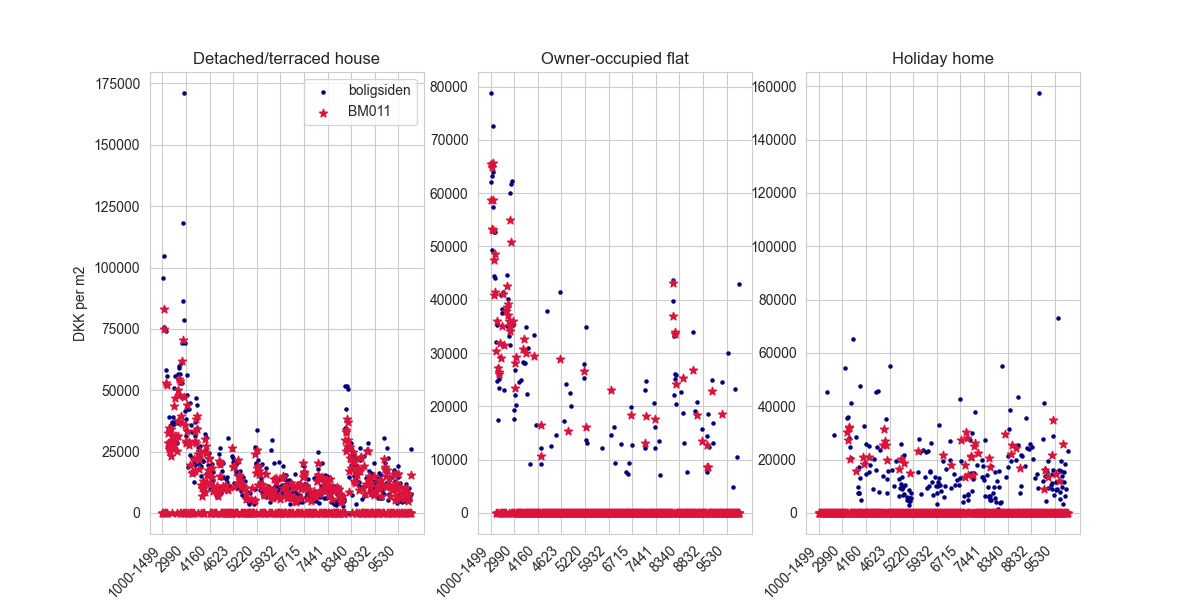
\includegraphics[width=15cm, height=7cm]{fig/Comparison_BM011_scraped.png}
                \caption{Validating scrapped data with property price from Finans Denmark}
                \label{fig:compar}
            \end{figure}    

        Figure \ref{fig:compar} plots the mean price per squared meter by three house types: Detached/ terraced house, owner-occupied flat, and holiday home over postal areas across Denmark. The \texttt{BM011} data is of 2023Q1 and the boligsiden data is up-to-date. Detached/ terraced house takes up 70.68\% of observations, owner-occupied flat 19.34\%, and holiday home 9.97\%, also in accordance with the same proportion of each type of houses on sale under lable \texttt{UDB010}. By eyeballing, we can find that the two datasets behave similarly over all three types. Our scrapped data is most similar to the data-set in the detached house type, which constitutes the majority of our observations, and the least in holiday home, which should be a result of little sample size. However, in each case, we can find the two data-sets share the same high and low values in the same area. To sum up, it is safe to say that our data-set is representative of the housing market of Denmark to this date.

        
            

    \subsection{Key Statistics}
        Table \ref{tab:summary_stats} presents the statistical measures pertaining to the chosen variables. It is evident that there exists a substantial disparity in real estate prices. Specifically, the range spans from a minimum of 20,000 DKK to a maximum of 78,000,000 DKK. The average and median prices converge around 3,000,000 DKK. Similarly, the variances in living space and number of rooms are notably extensive, likely attributable to the diverse array of real estate types. Houses generally encompass larger spatial dimensions compared to apartments, and houses typically incorporate a greater number of rooms. Figure \ref{fig:size_type} and \ref{fig:room_type} shows non-apartment (value = 0) have larger median dimensions and rooms than apartment (value = 1)

        \begin{table}[htbp]
        \centering
        \begin{tabular}{lccc}
        \toprule
        Metric & price & living\_space & rooms \\
        \midrule
        Mean & 3100033.7 & 141.34 & 4.55 \\
        Standard Deviation & 3387762.9 & 60.65 & 1.76 \\
        Minimum & 200000 & 10 & 1 \\
        25\% Percentile & 1375000 & 102 & 3 \\
        50\% Percentile (Median) & 2295000 & 134 & 4 \\
        75\% Percentile & 3795000 & 169 & 5 \\
        Maximum & 78000000 & 683 & 18 \\
        \bottomrule
        \end{tabular}
        \caption{Summary Statistics}
        \label{tab:summary_stats}
        \end{table}

        \begin{figure}[]
            \centering
            \includegraphics[scale=0.5]{fig/price_cop.png}
            \caption{price in different areas}
            \label{fig:price_cop}
        \end{figure}

        \begin{figure}[]
            \centering
            \includegraphics[scale=0.5]{fig/size.png}
            \caption{sizes of different types}
            \label{fig:size_type}
        \end{figure}

        \begin{figure}[]
            \centering
            \includegraphics[scale=0.5]{fig/room.png}
            \caption{rooms of different types}
            \label{fig:room_type}
        \end{figure}

        \begin{figure}[]
            \centering
            \includegraphics[scale=0.5]{fig/lv_p.png}
            \caption{relationship between size and price}
            \label{fig:price_size}
        \end{figure}

        In Figure \ref{fig:price_cop}, an evident disparity emerges as the median price of real estate within Copenhagen city (value = 1) surpasses that of other regions (value = 0). In contrast, other areas exhibit a considerable number of instances with notably elevated prices. It is presumed that these instances may owe their high prices to their remarkably expansive dimensions. As depicted in Figure \ref{fig:price_size}, a discernible relationship materializes between the price and the size of properties. Remarkably expensive properties often boast substantial dimensions; notably, these properties find themselves situated outside the confines of Copenhagen city.


\section{Methods}
	   We trained two machine learning models on residential housing prices in Denmark at the moment in each region. The feature variables include structural features such as house area and age and energy type, and external variables include location. The train and test datasets are split in a 70:30 way due to the limitation of available observations.\par

        % In model comparison, we make a model pipeline to fit training data. In cleaning data, we have done data pre-processing to make it suitable for training machine learning models. Then, we do feature engineering involves selecting, constructing, and transforming features to help the model better capture patterns and relationships in the data. After several models training, we evaluate the performance of the model.\par

    \subsection{Polynomial Model}
        The first model we trained is a 3-degree polynomial model with LASSO regularization and 10-fold cross-validation. This is the common practice in the literature in the prediction of housing prices not only because of its simplicity but also because of the fact that we can easily examine how each feature contributes to the prediction by inspecting the coefficients of the model. We minimize the standard workhorse LASSO formula
        \begin{equation}
            L_{LASSO}(\hat{\beta}) = \sum_{i=1}^n (y_i - \hat{y_i}(\beta))^2 + \lambda \sum_{j=1}^p |\hat{\beta}_j|
        \end{equation}
        where $\lambda$ is the penalty hyperparameter which we are going to tune with cross-validation.

		We examine the under-fitting and over-fitting problems by inspecting the learning curve and validation curve of linear regression.\par

    \subsection{Gradient Boosting Model}
        Following a vast literature implementing machine learning algorithms on the prediction of housing prices such as \cite{Linetal2023} and \cite{Deppneretal2023}, the second model we applied is the gradient boosting model (GBM) as it is arguably the most efficient and effectively predictive algorithm in the prediction of house prices. We also conducted 10-fold cross-validation by splitting the data into 10-fold even-sized validation bins. For each bin fit the model on the data outside the validation bin. We transform and predict the target in the validation bin. We pick the model which performed the best on the validation data during cross-validation.

       The gradient boosting model is a type of ensemble method combining different regressors that have better generalization performance than each individual regressor. As a boosting model, gradient boosting boosts weak learners to strong learners. It is different from adaptive learning with regard to how weights are updated and how weak regressors are combined. We follow the algorithm given in \cite{Raschka2019} in Chapter 7 and the authors' lecture note on ensemble models on \url{https://pages.stat.wisc.edu/~sraschka/teaching/stat479-fs2019/}.\par

       Gradient boosting model works as follows:
       \begin{enumerate}
           \item Construct a base tree by computing the prediction with the average of all training examples: 
           \begin{equation}
               \hat{y_1} = \frac{1}{n}\sum^n_{i=1} y^{(i)}
           \end{equation}
           and compute $$
           h_0(\textbf{x}) = \argmin_{\hat{y}}\sum^n_{i=1}L(y^{(i)}, \hat{y})$$ where $L(y^{(i}),h(\textbf{x}^{(i)}))$ is a pre-chosen differentiable loss function
           \item Build next tree based on errors of the previous tree: first with pseudo residual
           \begin{align}
               r_1 &= y_1 - \hat{y_1} \\
                &= -[\frac{\partial L(y^{(i)}, h(\textbf{x}^{(i)}))}{\partial h(\textbf{x}^{(i)})}]_{h(\textbf{x}^{(i)})=h_{t-1}(\textbf{x}^{(i)})}
           \end{align}
           where the second equation is the general form. And secondly, build a new decision tree for the residuals with terminal nodes $R_{j,t}$ where $j=1,...,J_t$.
           \item Combine trees from step 1 and 2, predict one entry with
           \begin{align}
               \hat{y_2} &= \hat{y_1} + \eta * r_1\\ &= \argmin_{\hat{y}}\sum_{\textbf{x}^{(i)}\in R_{i,j}}L(y^{(i)}, h_{t-1}(\textbf{x}^{(i)})+\hat{y}),
           \end{align}
           where $\eta$ is the learning rate, and the second equation is the general form. And then go to step 2 and compute
           \begin{equation}
               r_{2, 2} = y_2 - \hat{y_2}
           \end{equation}
           where $r_{i,t}$ is the pseudo residual of the $t$-th tree and $i$-th example and update
           \begin{equation}
               h_t(\textbf{x}) = h_{t-1}(\textbf{x}) + \eta * \sum_{j=1}^{J_t} \hat{y_{j,t}} \mathbb{I}(\textbf{x}\in R_{j,t})
           \end{equation}
           The procedure is repeated until meet the maximum depth of tree. The model returns the final $h_t(\textbf{x})$.
       \end{enumerate}

        We evaluate the predictive efficacy of models with R-squared and Root Mean Square Error (RMSE). We also inspect the importance of each feature in predicting the housing price. It turns out that GBM model outperforms linear model by 3 times in terms of RMSE and its R-squared is around 40\% higher than linear models.\par
		
\section{Empirical Analysis}
        In applying the model, certain features are omitted or included for better performance. Figure \ref{fig:heatmap} shows the correlation matrix of independent variables. Most variables are safely uncorrelated. Villa and land are more correlated to ground space due to the obvious reason that compared to holiday home, flat and detached house, these two types are more likely to have bigger ground place. However, we keep the two variables because we believe that they have separate predictive power. It should be noted as well that we include age squared in the linear regression as common practice to reduce bias. It is highly correlated to the feature 'age' but no concern should be raised. And figure \ref{fig:heatmapcat} shows the correlation matrix of categorical features used as coded but not explicitly in the form of dummy variables. The conclusion is generally the same as above. Following we introduce the results of our prediction models. Throughout the models, the random seed is set at 17082023, the starting date of our machine-learning exercise.
        
        \begin{figure}[]
            \centering
            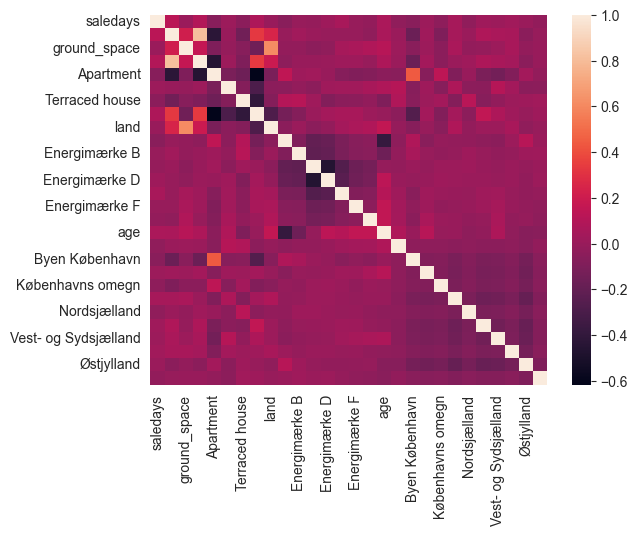
\includegraphics[scale=0.7]{fig/Xvar_corr_heat_map.png}
            \caption{Heatmap of X variables correlation matrix}
            \label{fig:heatmap}
        \end{figure}

        \begin{figure}[]
            \centering
            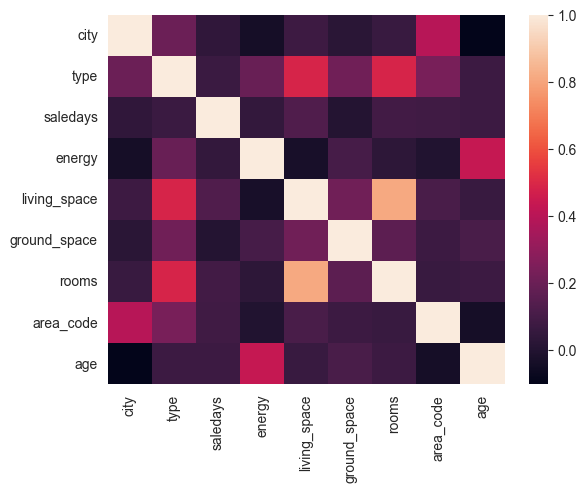
\includegraphics[scale=0.7]{fig/Xvar_corr_heat_map_cat.png}
            \caption{Heatmap of X variables correlation matrix}
            \label{fig:heatmapcat}
        \end{figure}

        \subsection{Polynomial Model}
        A common starting point in modeling house prices in the literature is polynomial linear regression. We conduct a 3-degree polynomial linear regression. We also conduct LASSO regularization penalizing parameters to tackle the problem of over- and under-fitting and run 10-fold cross-validation to tune for the best hyperparameter $\lambda$ given the small size of our dataset. We select root mean squared errors as the criteria. Figure \ref{fig:LASSOCVoripredtwo} plots the original and predicted test data with optimal hyperparameters given in table \ref{table:hyperparaLASSO}, and the line is a diagonal line. We can see that the LASSO model behaves largely unsatisfactory in prediction in the LHS. After dropping 746 \texttt{NaN} values and 3 outliers (larger than $10^8$), the prediction is much more satisfactory, as is shown in the RHS of figure \ref{fig:LASSOCVoripredtwo}, though it can be criticized that too many observations are omitted.

            \begin{figure}
                \centering
                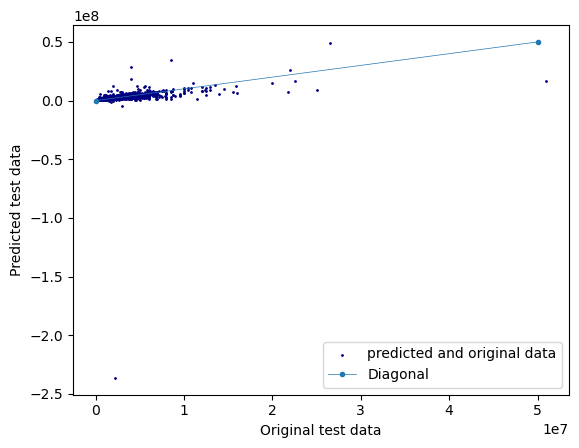
\includegraphics[width=.5\linewidth]{fig/LASSOCV_ori_vs_pred.png}\hfill
                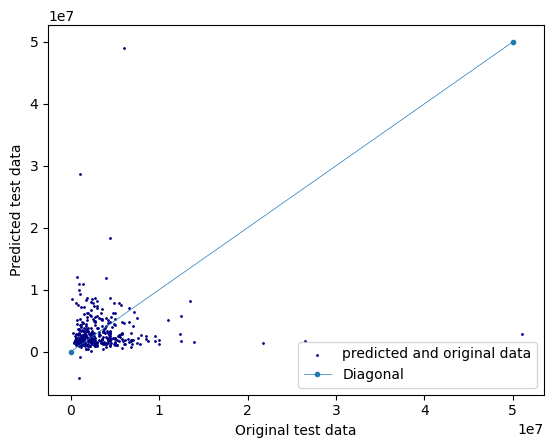
\includegraphics[width=.5\linewidth]{fig/LASSOCV_ori_vs_pred_drop.png}
                \caption{Original and Predicted data in optimal LASSO}
                \label{fig:LASSOCVoripredtwo}
            \end{figure}

		
		We test 66 evenly-distributed $\lambda$ from $10^{-4}$ to $10^4$ in LASSO and conducted 10-fold cross-validation. The best hyperparameter from LASSO and cross-validation and the corresponding RMSE from validation against each hyperparameter tuned is given in table \ref{table:hyperparaLASSO}. Note that the $\lambda$'s are extrema, and therefore the real optimal value may be out of our chosen scale. This means that we need higher penalty for parameters and more unimportant features are pushed to zero. This raises bias in tackling overfitting and may cause underfitting. We will further look into this with learning and validation curves.
  
            \begin{table}[]
            \begin{tabular}{lrr}
                             & \multicolumn{1}{l}{\textbf{Lambda}} & \multicolumn{1}{l}{\textbf{Validation RMSE}} \\ \hline
                3-degree Lasso               & 10,000.00                           & 249,834,112.73                               \\
                3-degree Lasso w/ 10-fold CV & 10,000.00                           & 8,438,023.01                                 \\ \hline
                \end{tabular}
            \caption{Tuned Hyperparameters for LASSO and LASSO with 10-fold CV}
            \label{table:hyperparaLASSO}
            \end{table}
            
            \subsubsection{Learning Curve}
            We examine the learning curve to find out if our model faces overfitting (high variance) or under-fitting (high bias) problem (pp.201-6, \cite{Raschka2019}). In figure \ref{fig:learcurve}, the x-axis is the training data size, and the y-axis is the model training and validation accuracies. The train dataset plot remains flat through the change in train size, whereas the root mean squared error of the test data dampens quickly around 300-400 data points, remains flat, and converges to the train plot with the increase of train size. This implies that with the increase in train size with more datapoints, we can expect our model to behave generally well in predicting housing prices in Denmark.

            \begin{figure}[]
                \centering
                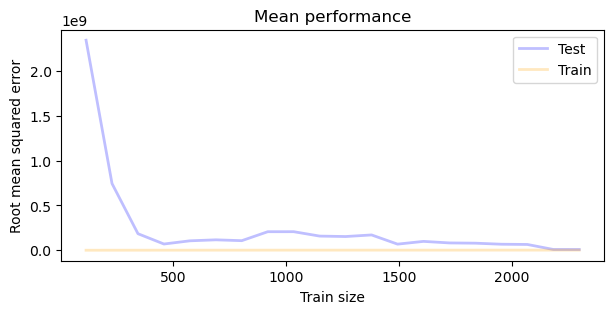
\includegraphics[width=.7\linewidth]{fig/LASSO_learning_curve.png}
                \caption{Learning Curve}
                \label{fig:learcurve}
            \end{figure}

            \subsubsection{Validation Curve}
            We also leverage the validation curve to address over- and under-fitting in figure \ref{fig:valcurve}. The y-axis is the same as the learning curve, while the x-axis is the model hyperparameters. The RMSE falls tremendously when $\lambda$ is larger than 1000, and converges to the training data. This indicates that with a higher strength of regularization, we can expect a higher accuracy of prediction.

            \begin{figure}[]
                \centering
                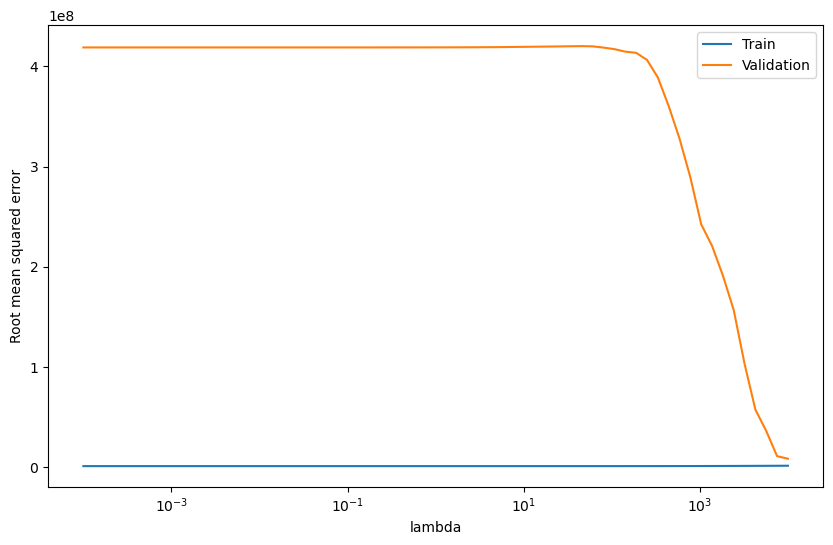
\includegraphics[width=.7\linewidth]{fig/LASSO_validation_curve.png}
                \caption{Validation Curve}
                \label{fig:valcurve}
            \end{figure}

        \subsection{Gradient Boosting Model}
            In practice, the histogram-based gradient boosting model is an enhanced model of gradient boosting \texttt{GradientBoostingRegressor} (GBM) in scikit-learn toolkit by the name of \texttt{HistGradientBoostingRegressor} (HGBM). It runs faster than ordinary gradient boosting but does not support the search for feature importance. However, the first does not support categorical features. We also experimented with \texttt{XGBRegressor} (XGB) which is essentially the same gradient boosting model yet faster and more memory-efficient and more importantly, supports both categorical features and feature importance plotting.\par
            
            The first two models are tuned against \texttt{max\_depth}, \texttt{learning\_rate} and \texttt{min\_samples\_leaf}. The \texttt{max\_depth} refers to the maximum depth of the tree we build. The deeper, the more splits we have and the more we learn from the predictors. We tune against [1, 2, 3, 4]. And the \texttt{learning\_rate} shrinks the contribution of each tree by the designated amount. With a higher learning rate, we are more likely to meet the over-fitting problem. We tune it in the range [0.1, 0.2, 0.4, 0.6, 0.8, 1, 1.2, 1.4, 1.6]. \texttt{min\_samples\_leaf} controls the minimum number of samples required to be at a leaf node. It has the effect of smoothing the model and is used to control the overfitting problem. We tune against [10, 30, 50, 70, 90]. There is no \texttt{min\_samples\_leaf} for \texttt{XGBRegressor} and thus we tune it against \texttt{max\_leaves}, meaning the maximum number of leaves, which is essentially the reciprocal of \texttt{min\_samples\_leaf}. We tune it against [0, 20, 40, 60, 80, 100].\par
            
            We can refer to table \ref{table:hyperparaGBM} for the optimal hyperparameters. We tested the three types of gradient boosting models. We tested ordinary GB with city as a categorical variable, XGB with city and zip, and HGBM with city, zip, and city and zip combined.\par
            
            The maximum tree depth of histo-based gradient boosting is 1, which is the smallest possible value, indicating that the model opts for a simple and shallow tree model. The optimal value of the maximum leaf for XGB is 0, which means no restriction is put on the maximum number. In all cases, the learning rate is the extremum in our tuning scale. This means that models tend to learn more from each tree and raises the worry of overfitting. 

            \begin{table}[h]
                \begin{tabular}{llll}
                \textbf{} & \textbf{Max depth} & \textbf{\begin{tabular}[c]{@{}l@{}}Min samples leaf/ \\ Max leaf\end{tabular}} & \textbf{Learning rate} \\ \hline
                GB w/ city                      & 2 & 90 & 1.6 \\
                Extreme GB w/ city \& zip       & 2 & 0  & 1.6 \\
                Histo GB w/ city          & 2 & 70 & 1.6 \\
                Histo GB w/ zip           & 1 & 1  & 1.6 \\
                Histo GB w/ city \&   zip & 2 & 70 & 1.6 \\ \hline
                \end{tabular}
            \caption{Tuned Hyperparameters for gradient boosting models with 10-fold CV}
            \label{table:hyperparaGBM}
            \end{table}

            Figure \ref{fig:HGBMoripred} plots the original and predicted test data from HGBM with city with optimal hyperparameters given in table \ref{table:hyperparaGBM}, and the line is diagonal line. We can see that the GBM behaves largely well in prediction.
            
            \begin{figure}[]
                \centering
                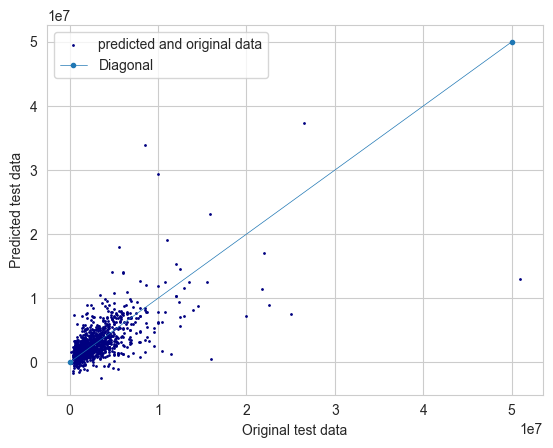
\includegraphics[width=.7\linewidth]{fig/HGBM_ori_vs_pred.png}
                \caption{Original and Predicted data in optimal HGBM}
                \label{fig:HGBMoripred}
            \end{figure}
            

                \subsubsection{Contribution of features}
                In figure \ref{fig:featurecontriGBM} we can find the importance of each feature to the final prediction in an optimal GBM \texttt{GradientBoostingRegressor}. We find that the feature that contributes the most is living space, which contributes about 48\%. The second is Nordsjælland, which contributes 11\%. This means that there is a substantial difference in housing prices between Nordsjælland and other parts of Denmark.\par
                
                In figure \ref{fig:featurecontriXGB} we can find the importance of each feature to the final prediction in a baseline XGB \texttt{XGBRegressor} with default parameters, which as we shall later see is the best model in prediction. We find that the feature that contributes the most to the prediction is the living space with 39\% importance. The second largest is zip code by about 29\% and following rooms, city, and energy all around 7\%.
                
            \begin{figure}[]
                \centering
                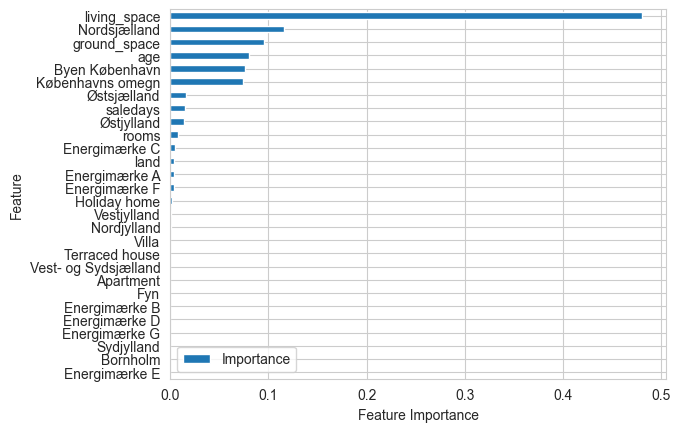
\includegraphics[scale=0.7]{fig/GBM_feature_importance.png}
                \caption{Optimal GBM feature importance}
                \label{fig:featurecontriGBM}
            \end{figure}
            
            \begin{figure}[]
                \centering
                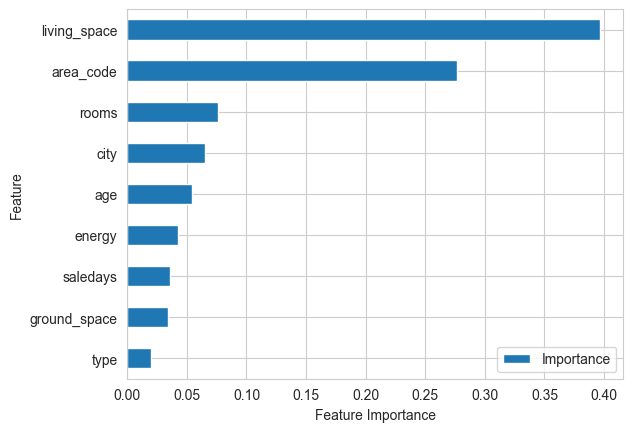
\includegraphics[scale=0.7]{fig/XGB_feature_importance-baseline_cat.png}
                \caption{Baseline XGB feature importance}
                \label{fig:featurecontriXGB}
            \end{figure}        
            
        \subsection{Model Comparison}
            We compare the root mean squared errors (RMSE) and r-squared (R2) of each model to see how well they perform in prediction. Table \ref{table:Model_comparison} concludes the relative performance of each model in a baseline with default parameters and optimal parameters after 10-fold cross validation. We can find that gradient-boosting models outperform LASSO models by around 3 times in terms of RMSE. The best-performing model is baseline \texttt{XGBRegressor}, with 0.44 R2 score, indicating that we can explain and predict 44\% of the variations in the residential real estate prices in Denmark, whereas polynomial regressions hardly have an R2 value. The second best is the histogram-based gradient boosting model with city as a dummy variable. The reason why models with \texttt{area\_code} as dummy variable is not the best, though it is a more detailed variable and in intuition is a better predictive feature in the housing prices, is the limit of available data. For each area code, there are only about 1-5 observations, which tremendously increases the variation and uncertainty of prediction. We can overcome this by increasing the dataset size.

            \begin{table}[h]
                \begin{tabular}{lrr}
                \textbf{Model   comparison} & \multicolumn{1}{l}{\textbf{RMSE}} & \multicolumn{1}{l}{\textbf{R\_2}} \\ \hline
                3-degree polynomial Linear                           & 1.74E+19     & 0.05   \\
                3-degree Lasso                                       & 7,619,160.64 & 0.05   \\
                3-degree Lasso w/ 10-fold CV                         & 7,619,160.64 & -      \\
                Gradient boosting w/ city baseline                   & 2,643,662.58 & 0.28   \\
                Gradient boosting w/ city optimal                    & 2,458,819.78 & 0.38   \\
                \textbf{Extreme gradient boosting baseline}                   & \textbf{2,329,683.66} & \textbf{0.44}   \\
                Extreme gradient boosting optimal                    & 2,806,964.29 & 0.19   \\
                Histo-based gradient boosting w/ city   baseline     & 2,442,247.15 & 0.39   \\
                Histo-based gradient boosting w/ city   optimal      & 2,697,510.92 & 0.25   \\
                Histo-based gradient boosting w/ zip-code   baseline & 3,102,302.28 & 0.01   \\
                Histo-based gradient boosting   w/ zip-code optimal  & 3,249,872.72 & (0.09) \\ \hline
                \end{tabular}
                \caption{Model Performance Comparison}
                \label{table:Model_comparison}
                \end{table}


\section{Discussion}
    \subsection{Comparison with Previous Studies} 
    
    Our findings corroborate and extend the results of prior research that has emphasized the significance of energy consumption in house valuation. The house price is notably impacted by various factors, particularly the living space, along with other significant influences like the city, group space, house age, house rooms, and house type. Among these, living space tends to wield a particularly strong influence on the overall pricing dynamics.
    
    \subsection{Limitations and Future Research Directions} 
    
    While our study provides valuable insights, it is essential to acknowledge its limitations. 
    
    Limited dataset size makes our models may attempt to fit noise in the data. There are several reasons for the insufficient data volume.The boligsiden website shows there are totally 47,728 houses for sale, however, we can only see 200 pages which is 10,000 houses observations. During the scraping process, we encountered certain challenges. Specifically, when attempting to scrape the "energy ranking" variable, our code consistently encountered errors. The specific error message received was "'NoneType' object has no attribute 'text'". Within our code, we've successfully managed to scrape observations without encountering errors within a loop. However, it's worth noting that due to the error encountered during the scraping of the "energy ranking" variable, our overall data collection process has been constrained, resulting in a reduced number of observations obtained.
    
    The relative location of the houses is not considered because we do not have enough time to get relative location data in hvorlangterder.dk. Real estate markets can exhibit significant price variations within relatively small geographic areas. Failing to account for local market dynamics can result in generalized and imprecise price predictions that don't accurately reflect the intricacies of the neighborhood or district. The optimal approach to our feature selection, would be using relative location data in hvorlangterder.dk.
    


    \subsection{Practical Implications}
    
    Using machine learning to predict house price in Denmark can benefit a lot for buyers and sellers in the real estate market. Prospective buyers, armed with accurate price predictions, can make well-informed choices aligned with their budget and preferences, leading to more satisfying property acquisitions. Sellers can strategically price their properties based on data-driven insights, optimizing their listing strategies to attract potential buyers effectively. Moreover, our predictive model can be leveraged by policymakers, real estate professionals to make informed decisions. 

    
\section{Conclusion}
    We web-scraped up-to-date residential real estate prices and features in Denmark from leading danish real estate broker boligsiden to perform machine learning exercises to predict the prices of housing prices in Denmark. Our workhorse model is a traditional hedonic model, with internal features such as living space and rooms, and external features such as location and days on sale. We successfully scraped 7619 observations from a list of 10000 website links, and conducted thorough data cleaning to get a final data set of 3754 entries.
    
    We executed machine learning with polynomial regression with LASSO, and gradient boosting models, both with 10-fold cross-validation. Our research shows that a tuned gradient boosting model with scikit-learn function \texttt{XGBRegressor} can best predict housing prices with a satisfactory R2 score of 44\% and RMSE of 2,329,683.66. The feature that contributes the most to prediction is living space, with an importance score of 39\% and the second is zip code at 29\%. Further exercise can extend to obtaining more observations and including more features to improve prediction accuracy.

\newpage
\footnotesize
\bibliographystyle{apalike}
\bibliography{Project}


\section{Appendix}


\begin{table}[htbp]
\centering
\begin{tabular}{m{2.5cm} m{5cm} c c}
\toprule
Variable & Description & Transformed to Dummy Variables & Dropped \\
\midrule
city & City names & TRUE & FALSE \\
energy & Energy ranking from A to G & TRUE & FALSE \\
area\_code & Zip code & TRUE & FALSE \\
type & Housing type & TRUE & FALSE \\
expenses & Owner expense every month & FALSE & TRUE \\
living\_space & Size & FALSE & FALSE \\
address & Street and number & FALSE & TRUE \\
saledays & Days after sale & FALSE & FALSE \\
ground\_space & Size of land & FALSE & FALSE \\
rooms & Number of rooms & FALSE & FALSE \\
age & Housing age & FALSE & FALSE \\
\bottomrule
\end{tabular}
\caption{Variable Descriptions and Handling}
\label{tab:variables}
\end{table}




\end{document}
